%-----------------------------------------------------------------------------%
\chapter{\babEmpat}
%-----------------------------------------------------------------------------%


Bab ini menjelaskan tentang perancangan sistem rekomendasi lokasi pencacahan yang diusulkan. Sebelum dijelaskan tentang sistem usulan, terlebih dahulu akan dilakukan eksperimen dan analisis terhadap solusi yang telah ada.


%-----------------------------------------------------------------------------%
\section{Analisis}
\label{sec:analysis}
%-----------------------------------------------------------------------------%
Pada kondisi saat ini, lokasi pencacahan sudah ditentukan sejak awal dengan menggunakan metode sampling tertentu. Pada tahap perancangan, petugas direkrut dan dialokasikan ke lokasi pencacahan terdekat. Pengalokasian seringkali dilakukan secara subyektif berdasarkan kedekatan lokasi pencacahan dengan domisili petugas pencacahan. Akibatnya, terjadi ketidakmerataan beban kerja dan variasi total waktu penyelesaian pekerjaan yang sangat tinggi antar petugas. 

Untuk mengatasi masalah ini, algoritma MDVRP dipilih sebagai metode pemecahan masalah karena memiliki karakteristik yang serupa dengan permasalahan alokasi petugas, yakni: 

\begin{enumerate}
	\item Terdapat lebih dari satu \textit{vehicle}, dimana masing-masing vehicle memiliki \textit{depot} yang berbeda. Ini analog dengan permasalahan alokasi petugas, dimana ada lebih dari satu pencacah dan masing-masing pencacah memiliki titik mulai pencacahan yang berbeda. 
	\item Terdapat \textit{cost} yang harus dikeluarkan untuk melakukan perjalanan dari satu customer ke customer yang lain. Ini sejalan dengan konsep dalam pencacahan dimana terdapat \textit{cost} untuk mengunjungi satu responden ke responden lainnya. 
\end{enumerate}

Dalam proses pencacahan, \textit{cost} dapat berupa waktu tempuh, jarak tempuh, atau biaya perjalanan. Dalam penelitian ini, waktu tempuh dipilih sebagai representasi dari \textit{cost} karena waktu tempuh menggambarkan tingkat kesulitan akses untuk tiap-tiap responden. Semakin sulit akses ke suatu wilayah, semakin lama waktu tempuh yang diperlukan. 

Eksperimen dilakukan untuk membuktikan fisibilitas MDVRP dalam penyelesaian permasalahan alokasi petugas, dengan melibatkan 2 (dua) komponen utama:
\begin{enumerate}
	\item Sejumlah pencacah yang masing-masing memiliki \textit{depot} tersendiri. 
	\item Sejumlah lokasi pencacahan/blok sensus yang masing-masing terdiri dari beberapa responden. 
\end{enumerate}

Subbab \ref{ssec:mtsp_dataset} hingga subbab \ref{ssec:hasil-analisis} menyajikan penjelasan rinci mengenai langkah-langkah yang dilakukan dalam eksperimen. 

%-----------------------------------------------------------------------------%
\subsection{Dataset}
\label{ssec:mtsp_dataset}
%-----------------------------------------------------------------------------%
\subsubsection{Lokasi Pencacahan}
%-----------------------------------------------------------------------------%
Merujuk kepada konsep MDVRP, lokasi pencacahan dapat dianalogikan sebagai pelanggan (\textit{customer}) yang akan dikunjungi oleh petugas pencacah (\textit{vehicle}). Pengujian dilakukan dengan menggunakan data 182 lokasi nagari/kelurahan yang bersumber dari data wilayah administratif di Kabupaten Pesisir Selatan, Provinsi Sumatera Barat. Masing-masing lokasi memiliki atribut ID dan posisi menurut garis lintang dan bujur, seperti yang terlihat pada \autoref{tbl:enumeration_locations}.


\begin{table*}[!]
	\centering
	\ra{1.3}
	\caption{Lokasi Pencacahan}
	\label{tbl:enumeration_locations}
	\begin{tabular}{lcc}
		\toprule
		& \multicolumn{2}{c}{Koordinat}\\
		\cmidrule{2-3}
		& Latitude & Longitude\\ 
		\midrule
		1302011001 & -2.3504 & 101.1434\\ 
		1302011002 & -2.4233 & 101.0285\\ 
		1302011003 & -2.3798 & 101.0427\\ 
		1302011004 & -2.3884 & 101.049\\ 
		1302011005 & -2.3936 & 101.0546\\
		...\\
		1302110019 & -1.2387 & 100.4853\\ 
		1302110020 & -1.1408 & 100.4938\\ 
		1302110021 & -1.0883 & 100.4652\\ 
		1302110022 & -1.0886 & 100.489\\ 
		1302110023 & -1.1523 & 100.4978\\
		\bottomrule
	\end{tabular}
\end{table*}


%-----------------------------------------------------------------------------%
\subsubsection{Petugas Pencacahan}
%-----------------------------------------------------------------------------%
Berdasarkan konsep MDVRP, petugas pencacahan diibaratkan sebagai kendaraan yang harus berpindah dari satu lokasi ke lokasi lain secara berurutan. Selain memiliki atribut ID, masing-masing pencacah juga dilengkapi dengan atribut \textit{depot}, yaitu lokasi dimana pencacah harus memulai dan mengakhiri kunjungan. Eksperimen ini menggunakan 15 pencacah dengan lokasi \textit{depot} yang bervariasi, seperti contoh yang tercantum pada \autoref{tbl:enumerator}.


\begin{table*}[!]
	\centering
	\ra{1.3}
	\caption{Pencacah}
	\label{tbl:enumerator}
	\begin{tabular}{lcc}
		\toprule
		& \multicolumn{2}{c}{Koordinat Depot}\\
		\cmidrule{2-3}
		& Latitude & Longitude\\ 
		\midrule
		1302011008 & -2.3905 & 101.1214\\
		1302012003 & -2.199 & 101.1188\\
		1302020006 & -2.1225 & 101.0687\\
		...\\
		1302100002 & -1.23265 & 100.54314\\
		1302101005 & -1.19831 & 100.58078\\
		1302110003 & -1.2475 & 100.4745\\
		\bottomrule
	\end{tabular}
\end{table*}


%-----------------------------------------------------------------------------%
\subsubsection{Jarak dan Waktu Tempuh}
\label{ss:distance-duration-matrix}
%-----------------------------------------------------------------------------%
Jarak dan waktu tempuh antar lokasi pencacahan digunakan sebagai penimbang dalam penentuan rekomendasi lokasi. Penghitungan jarak dan waktu tempuh dapat dilakukan dengan cara manual (menggunakan hasil survei dan perkiraan \textit{subject matter}) atau memanfaatkan \textit{Google Directions API} \citep{google_google_2016}. 


Secara teknis, \textit{Google Direction API} lebih unggul dibandingkan metode manual karena telah otomatis mengikutsertakan faktor rute tercepat, kondisi geografis, moda transportasi yang digunakan, dan kemacetan lalu lintas dalam kalkulasi jarak dan waktu tempuh. Namun, \textit{Google Direction API} menggunakan informasi yang bersumber dari kontribusi para pengguna \textit{Google}, sehingga ada kemungkinan rute-rute yang jarang dilewati akan memiliki informasi yang minim. Sebagai konsekuesinya, terdapat resiko hasil kalkukasi yang bias untuk rute-rute tersebut. 


Kode \autoref{lst:google_direction_api_request} menggambarkan contoh \textit{requests URL} yang dikirimkan ke \textit{Google Direction API}. \textit{Request URL} ini dapat dieksekusi dengan menggunakan \textit{HTTP client}, seperti \textit{curl} dan \textit{wget}, atau \textit{HTTP client library}, seperti \textit{requests} dan \textit{urllib} di Python. Contoh \textit{response} Google Direction API dapat dilihat pada Gambar \ref{fig:google_direction_api_response}.


Hasil kalkulasi jarak dan waktu tempuh kemudian disimpan dalam bentuk matriks seperti yang terlihat pada Tabel \ref{tbl:distance_duration_matrix}. Jika lokasi \textit{depot} dari pencacah tidak tercakup dalam lokasi pencacahan yang ada, maka lokasi \textit{depot} tersebut harus ditambahkan ke dalam matriks jarak dan waktu tempuh.


\begin{listing}[!]
	\caption{Google Direction API Request}
	\label{lst:google_direction_api_request}
	\begin{minted}[showspaces=false, breaklines=true]{http}
https://maps.googleapis.com/maps/api/directions/json?origin=origin_lat,
origin_lon&destination=dest_lat,dest_lon&departure_time=timestamp&
traffic_model=best_guess&key=API_KEY
	\end{minted}
\end{listing}


\begin{figure}[!]
	\centering
	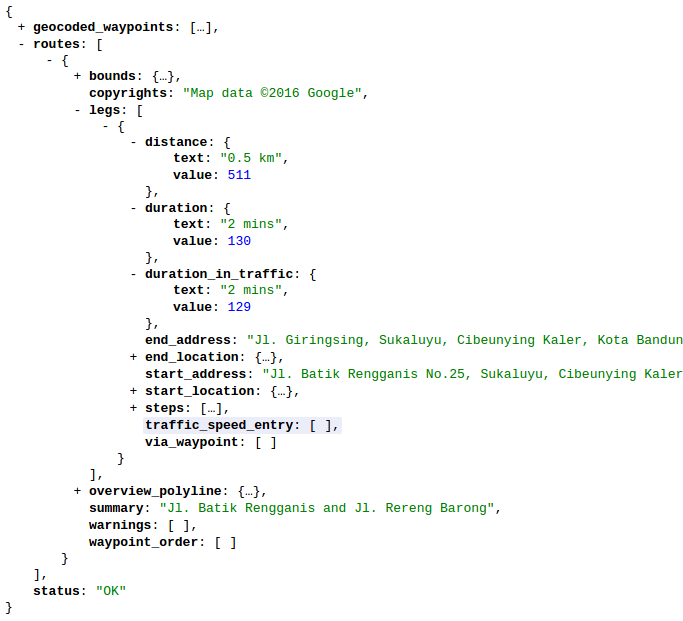
\includegraphics[width=\textwidth]{Resources/Images/google_direction_api_response}
	\caption{Google Direction API Response}
	\label{fig:google_direction_api_response}
\end{figure}


\begin{table}[!]
	\centering
	\ra{1.3}
	\caption{Data Jarak dan Waktu Tempuh}
	\label{tbl:distance_duration_matrix}
	\begin{tabular}{llcc}
		\toprule
		Lokasi A & Lokasi B & Jarak (m) & Waktu Tempuh (det)\\
		\midrule
		1302021001 & 1302021003 & 11119 & 1055\\
		1302021001 & 1302021002 & 9373 & 868\\
		1302021001 & 1302021005 & 490 & 38\\
		1302021001 & 1302021004 & 22760 & 2044\\
		...\\
		1302040015 & 1302012010 & 77889 & 8305\\
		1302040014 & 1302100015 & 103893 & 9984\\
		1302040014 & 1302012010 & 73561 & 7546\\
		1302100015 & 1302012010 & 171636 & 16801\\
		\bottomrule
	\end{tabular}
\end{table}


%-----------------------------------------------------------------------------%
\subsection{Algoritma dan Implementasi}
\label{ssec:alg-impl}
%-----------------------------------------------------------------------------%
Terdapat banyak \textit{library} yang dapat digunakan untuk mengatasi permasalahan MDVRP, baik yang berbayar maupun \textit{open source}. Dua \textit{open source library} yang cukup terkenal untuk permasalahan MDVRP adalah Jsprit \citep{jsprit_jsprit_2014} dan Optaplanner \citep{optaplanner_constraint_2016}. Eksperimen ini menggunakan JSpirit karena lebih berfokus pada \textit{route finding} serta lebih mudah untuk diimplementasikan. 


Jsprit merupakan sebuah library berbasis java yang digunakan untuk menyelesaikan permasalahan \textit{traveling salesman problem} (TSP) dan \textit{vehicle routing problems} (VRP). Jsprit mencakup berbagai skenario seperti : \textit{pickups and deliveries}, \textit{back hauls}, \textit{heterogeneous fleets}, \textit{finite and infinite fleets}, \textit{multiple depots}, \textit{time windows}, \textit{open routes}, \textit{different start and end locations}, \textit{multiple capacity dimensions}, \textit{initial loads}, \textit{skills}, dll. Jspirit bekerja secara terstruktur, mulai dari pendefinisan masalah, pemilihan algoritma, pencarian solusi, hingga pemilihan solusi terbaik.


%-----------------------------------------------------------------------------%
\subsubsection{Definisi Masalah}
%-----------------------------------------------------------------------------%
Pendefinisian masalah dengan library Jsprit dilakukan dengan mendefinisikan lokasi pencacahan, para pencacah, dan matriks jarak dan waktu tempuh yang diimplementasikan dalam Kode \ref{lst:jsprit_define_locations}, Kode \ref{lst:jsprit_define_enumerators}, dan Kode \ref{lst:jsprit_define_route_weights}. Ketiga variabel ini kemudian di-\textit{build} menjadi satu dengan menggunakan \textit{syntax} yang tercantum pada Kode \ref{lst:jsprit_build_problem}.


\begin{listing}[!]
	\caption{Definisi Lokasi Pencacahan}
	\label{lst:jsprit_define_locations}
	\begin{minted}[showspaces=false,breaklines=true]{java}
	Service.Builder builder = Service.Builder.newInstance(line[0]);
	
	try {
	Location loc = Location.Builder.newInstance()
	.setId(line[0])
	.setCoordinate(
	Coordinate.newInstance(Double.parseDouble(line[2]), 
	Double.parseDouble(line[1]))).build();
	builder.setLocation(loc);
	} catch (Exception e) {}
	
	Service node = builder.build();
	vrpBuilder.addJob(node);
	\end{minted}
\end{listing}


\begin{listing}[!]
	\caption{Definisi Pencacah dari File .csv}
	\label{lst:jsprit_define_enumerators}
	\begin{minted}[showspaces=false,breaklines=true]{java}
	VehicleTypeImpl.Builder vehicleTypeBuilder = VehicleTypeImpl.Builder.newInstance("enumerator");
	vehicleTypeBuilder.setCostPerDistance(0);
	vehicleTypeBuilder.setCostPerTransportTime(1);
	vehicleTypeBuilder.setCostPerServiceTime(1);
	VehicleType vehicleType = vehicleTypeBuilder.build();
	
	VehicleImpl.Builder builder = VehicleImpl.Builder.newInstance(line[0]);
	
	try {
	Location loc = Location.Builder.newInstance()
	.setId(line[0])
	.setCoordinate(Coordinate.newInstance(Double.parseDouble(line[2]),
	Double.parseDouble(line[1])))
	.build();
	builder.setStartLocation(loc);
	} catch (Exception e) {}
	
	
	builder.setType(vehicleType);
	VehicleImpl vehicle = builder.build();
	vrpBuilder.addVehicle(vehicle);
	\end{minted}
\end{listing}


\begin{listing}[!]
	\caption{Definisi Penimbang Jarak dan Waktu Tempuh dari File .csv}
	\label{lst:jsprit_define_route_weights}
	\begin{minted}[showspaces=false,breaklines=true]{java}
	VehicleRoutingTransportCostsMatrix.Builder costMatrixBuilder = VehicleRoutingTransportCostsMatrix.Builder
	.newInstance(true);
	
	while ((line = reader.readNext()) != null) {
	try {
	costMatrixBuilder.addTransportDistance(line[0], line[1], Double.parseDouble(line[2]));
	costMatrixBuilder.addTransportTime(line[0], line[1], Double.parseDouble(line[3]));
	} catch (Exception e) {
	costMatrixBuilder.addTransportDistance(line[0], line[1], 0.0);
	costMatrixBuilder.addTransportTime(line[0], line[1], 0.0);
	}
	}
	
	VehicleRoutingTransportCosts costMatrix = costMatrixBuilder.build();
	vrpBuilder.setRoutingCost(costMatrix);
	\end{minted}
\end{listing}


\begin{listing}[!]
	\caption{Build Problem}
	\label{lst:jsprit_build_problem}
	\begin{minted}[showspaces=false,breaklines=true]{java}
	VehicleRoutingProblem.Builder vrpBuilder = VehicleRoutingProblem.Builder.newInstance();
	vrpBuilder.setFleetSize(VehicleRoutingProblem.FleetSize.FINITE);
	VehicleRoutingProblem problem = vrpBuilder.build();
	\end{minted}
\end{listing}


%-----------------------------------------------------------------------------%
\subsubsection{Definisi Algoritma}
%-----------------------------------------------------------------------------%
Berdasarkan masalah yang telah didefinisikan sebelumnya, Jsprit kemudian akan menciptakan algoritma yang bersifat \textit{out of the box} sesuai dengan jumlah iterasi dan thread yang didefinisikan pada Kode \ref{lst:jsprit_create_algorithm}. 


\begin{listing}[!]
	\caption{Penentuan Algoritma}
	\label{lst:jsprit_create_algorithm}
	\begin{minted}[showspaces=false,breaklines=true]{java}
	VehicleRoutingAlgorithm algorithm = Jsprit.Builder.newInstance(problem)
	.setProperty(Jsprit.Parameter.THREADS, 5).buildAlgorithm();
	algorithm.setMaxIterations(iterations);
	\end{minted}
\end{listing}


%-----------------------------------------------------------------------------%
\subsubsection{Pencarian Solusi dan Penentuan Solusi Terbaik}
%-----------------------------------------------------------------------------%
Pencarian solusi dilakukan dengan menggunakan algoritma yang dihasilkan pada tahap sebelumnya. Jika algoritma memproduksi lebih dari satu solusi, maka Jspirit akan melakukan pemilihan solusi terbaik seperti yang terlihat pada Kode \ref{lst:jsprit_search_solution}. 


\begin{listing}[!]
	\caption{Pencarian Solusi}
	\label{lst:jsprit_search_solution}
	\begin{minted}[showspaces=false,breaklines=true]{java}
	Collection<VehicleRoutingProblemSolution> solutions = algorithm.searchSolutions();
	VehicleRoutingProblemSolution bestSolution = Solutions.bestOf(solutions);
	\end{minted}
\end{listing}


%-----------------------------------------------------------------------------%
\subsection{Hasil dan Analisis}
\label{ssec:hasil-analisis}
%-----------------------------------------------------------------------------%
Berdasarkan hasil dari eksperimen, diperoleh rekomendasi seperti yang diilustrasikan pada Gambar \ref{fig:analysis_mtsp_recommendation} dan Listing \ref{lst:analysis_mtsp_recommendation} untuk detail dari masing-masing pencacah. \textit{Service time} untuk masing-masing lokasi pencacahan dirancang untuk mengikuti distribusi \textit{normal}. Pengujian dengan menggunakan 182 lokasi pencacahan dan 15 pencacahan menghasilkan rata-rata dan standar deviasi waktu penyelesaian untuk masing-masing pencacah sebesar:   \color{red} \textbf{tambahkan supporting data. jangan lupa di-refer-kan}	\color{black}
$$ \mu = 82.24 jam $$
$$ \sigma = 88.95 jam $$


\begin{figure}[!]
	\centering
	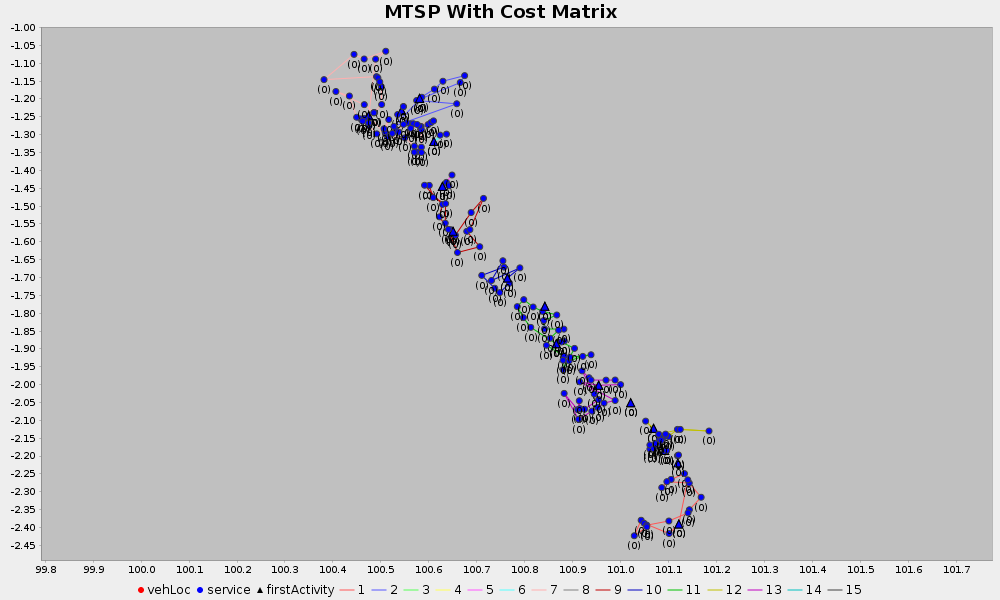
\includegraphics[width=\textwidth]{Resources/Images/analysis_mtsp_no_time_windows}
	\caption{Grafik Rekomendasi dengan MDVRP}
	\label{fig:analysis_mtsp_recommendation}
\end{figure}


\begin{listing}[!]
	\caption{Rekomendasi dengan MDVRP}
	\label{lst:analysis_mtsp_recommendation}
	\begin{minted}[showspaces=false,breaklines=true, escapeinside=||]{text}
	|\textbf{1302021005}| : 1302021001 --> 1302021005
	|\textbf{1302101005}| : 1302101005 --> 1302101001 --> 1302100010 --> 1302100014 --> 1302100011 --> 1302101004 --> 1302101006 --> 1302101003 --> 1302101002
	|\textbf{1302070006}| : 1302070006 --> 1302070002 --> 1302070003 --> 1302080009 --> 1302080004 --> 1302080001 --> 1302080005 --> 1302080003 --> 1302070012 --> 1302070011 --> 1302070001 --> 1302070004 --> 1302070007 --> 1302070008 --> 1302070010 --> 1302070009 --> 1302070005
	|\textbf{1302050007}| : 1302050007
	|\textbf{1302100002}| : 1302100002 --> 1302100003 --> 1302100013 --> 1302100012
	|\textbf{1302030005}| : 1302030005
	|\textbf{1302110003}| : 1302110003 --> 1302100001 --> 1302090006 --> 1302090012 --> 1302090003 --> 1302090014 --> 1302090009 --> 1302090015 --> 1302090018 --> 1302090016 --> 1302090017 --> 1302090013 --> 1302090005 --> 1302090007 --> 1302090002 --> 1302090008 --> 1302090001 --> 1302100015 --> 1302100004 --> 1302100016 --> 1302090011 --> 1302090010 --> 1302100017 --> 1302100006 --> 1302100007 --> 1302100009 --> 1302100008 --> 1302100005 --> 1302110001 --> 1302110010 --> 1302110013 --> 1302110002 --> 1302110014 --> 1302110015 --> 1302110011 --> 1302110016 --> 1302110017 --> 1302110004 --> 1302110018 --> 1302110019 --> 1302110005 --> 1302110012 --> 1302110023 --> 1302110020 --> 1302110006 --> 1302110007 --> 1302110008 --> 1302110021 --> 1302110009 --> 1302110022
	|\textbf{1302012003}| : 1302012007 --> 1302012003 --> 1302012008
	|\textbf{1302080006}| : 1302080006 --> 1302080008 --> 1302080002 --> 1302080007
	|\textbf{1302031005}| : 1302031005 --> 1302031008 --> 1302030014 --> 1302030006 --> 1302030009 --> 1302030004 --> 1302030010 --> 1302031003 --> 1302030002 --> 1302031004 --> 1302030003 --> 1302030012 --> 1302031001 --> 1302031006 --> 1302040011 --> 1302031009 --> 1302031010 --> 1302031002 --> 1302031007 --> 1302030001
	|\textbf{1302060005}| : 1302060005 --> 1302060009 --> 1302060006 --> 1302060008 --> 1302060002 --> 1302060007 --> 1302060001 --> 1302060003 --> 1302060004
	|\textbf{1302020006}| : 1302020006 --> 1302020015 --> 1302020011 --> 1302020009 --> 1302020010 --> 1302020001 --> 1302020003 --> 1302020005 --> 1302021006 --> 1302021002 --> 1302021007 --> 1302021008 --> 1302021003 --> 1302021009 --> 1302021004 --> 1302021010 --> 1302020016 --> 1302020017
	|\textbf{1302011008}| : 1302011008 --> 1302011007 --> 1302011004 --> 1302011003 --> 1302011002 --> 1302011006 --> 1302011005 --> 1302011009 --> 1302011010 --> 1302011001 --> 1302012005 --> 1302012002 --> 1302012009 --> 1302012010 --> 1302012004 --> 1302012001 --> 1302012006
	|\textbf{1302040002}| : 1302040002 --> 1302040003 --> 1302040004 --> 1302040015 --> 1302040008 --> 1302040009 --> 1302040010 --> 1302040014 --> 1302040012 --> 1302040013 --> 1302040001 --> 1302040016 --> 1302040007 --> 1302040006 --> 1302040005 --> 1302050001 --> 1302050004 --> 1302050006 --> 1302050002 --> 1302050008 --> 1302050010 --> 1302050009 --> 1302050005 --> 1302050003
	|\textbf{1302090004}| : 1302090004 --> 1302090019 --> 1302090020
	\end{minted}
\end{listing}


\begin{table}[!]
	\centering
	\ra{1.3}
	\caption{Total Waktu Setiap Pencacah dengan MDVRP}
	\label{tbl:enumerators_total_time}
	\begin{tabular}{lc}
		\toprule
		Pencacah & Total Waktu (jam)\\
		\midrule
		1302021005 & 13.3\\
		1302101005 & 60.8\\
		1302070006 & 116\\
		1302050007 & 6\\
		1302100002 & 26.6\\
		1302030005 & 6\\
		1302110003 & 341\\
		1302012003 & 19.9\\
		1302080006 & 27.1\\
		1302031005 & 136\\
		1302060005 & 61.3\\
		1302020006 & 121\\
		1302011008 & 116\\
		1302040002 & 162\\
		1302090004 & 20.2\\
		\bottomrule
	\end{tabular}
\end{table}


Nilai standar deviasi yang tinggi menunjukkan terjadinya ketidakmerataan beban kerja antar pencacah. Ini sekaligus menunjukkan bahwa MDVRP kurang ideal untuk digunakan dalam penentuan rekomendasi. Hal ini terjadi karena MDVRP memproduksi solusi berupa \textit{precalculated routes} (rute yang harus dikunjungi dari awal hingga akhir tugas pencacahan) tanpa memperhitungkan faktor lamanya waktu kunjungan pada satu lokasi pencacahan (\textit{service time}). Data mengenai \textit{Service time} hanya akan tersedia jika suatu lokasi sudah selesai dikunjungi sehingga tidak bisa diikutsertakan dalam kalkulasi rekomendasi. \autoref{fig:illustration-timeline-mdvrp} menunjukkan ilustrasi penerapan MDVRP pada permasalahan alokasi petugas pencacahan yang dapat dijabarkan sebagai berikut:
\begin{enumerate}
	\item Terdapat 10 lokasi pencacahan yang harus dikunjungi. MDVRP men-\textit{generate} solusi berupa \textit{precalculated routes} untuk petugas A dan B, dimana masing-masing mendapatkan jumlah beban tugas yang sama besar, yakni 5 lokasi. 
	\item Petugas pencacahan A dan B sama-sama memulai tugas pada waktu $t_{s}$ (\textit{time start}) yang digambarkan sebagai segmen berwarna hijau.
	\item Petugas A dan B berjalan menuju lokasi pencacahan masing-masing (lokasi \textit{i}) yang memakan waktu selama $t_{i}$ (segmen berwarna putih). 
	\item Pada setiap lokasi \textit{i}, masing-masing petugas memerlukan waktu sebesar $t_{i.1}$ untuk menyelesaikan tugas pencacahan (segmen berwarna biru). 
	\item Petugas A dan B menyelesaikan tugas pada waktu $t_{f}$ (\textit{time finish}) yang digambarkan sebagai segmen berwarna merah muda. 
\end{enumerate}

Dari \autoref{fig:illustration-timeline-mdvrp}, terlihat bahwa kalkulasi rekomendasi rute tanpa melibatkan \textit{service time}, mengakibatkan $t_{i}$ dan $t_{i.1}$ yang tidak berimbang antara petugas A dan B. Petugas A mendapatkan rute dengan rata-rata \textit{service time} ($t_{i.1}$) yang lebih panjang sehingga $t_{f}$ petugas A menjadi lebih besar dibandingkan $t_{f}$ petugas B. Perbedaan yang paling signifikan terlihat pada lokasi pencacahan kedua dari masing-masing petugas. Petugas A memiliki $t_{2.1}$ yang hampir 3 (tiga) kali $t_{2.1}$ petugas B. Sebagai dampaknya, terjadi ketimpangan dalam total waktu penyelesaian pencacahan antar petugas, dimana beban tugas petugas A menjadi jauh lebih berat dibandingkan petugas B. 

\begin{figure}[!]
	\centering
	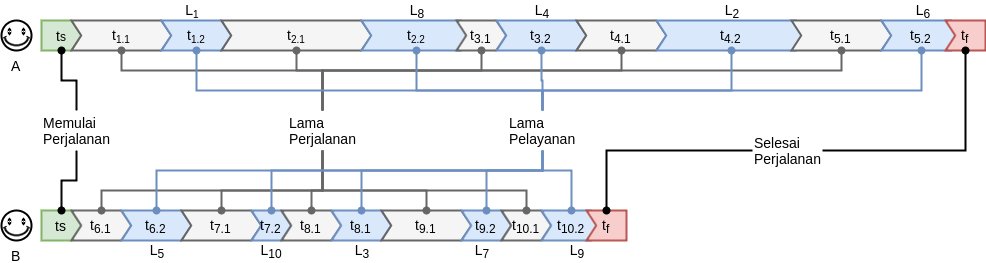
\includegraphics[width=\textwidth]{Resources/Images/illustration-timeline-mdvrp}
	\caption{Penerapan MDVRP pada Permasalahan Alokasi Petugas Pencacahan}
	\label{fig:illustration-timeline-mdvrp}
\end{figure}


Untuk mengatasi masalah ini diperlukan suatu mekanisme kalkulasi rekomendasi yang tidak terikat \textit{service time}. Mekanisme ini kemudian akan dikombinasikan dengan MDVRP sehingga menghasilkan suatu metode baru yang dapat menutupi kelemahan MDVRP sekaligus memberikan rekomendasi rute yang lebih adil kepada semua petugas pencacahan. 


%-----------------------------------------------------------------------------%
\section{Perancangan Solusi}
\label{sec:design}
%-----------------------------------------------------------------------------%
Hasil eksperimen pada \autoref{ssec:hasil-analisis} menunjukkan bahwa mekanisme kalkulasi yang \textit{independent} dari \textit{service time} diperlukan untuk menghilangkan bias dan kesenjangan rute untuk tiap-tiap petugas. Solusi yang diusulkan untuk mengatasi masalah ini adalah dengan melakukan penghitungan rute secara bertahap dengan melakukan `hibridisasi' antara algoritma MDVRP dengan suatu mekanisme \textit{real time}. Idenya adalah, daripada menghitung rute secara lengkap diawal pencacahan, lebih baik rute dihitung secara bertahap dan \textit{real time} dengan memanfaatkan \textit{current location} dari petugas sebagai depot yang baru pada setiap tahapnya. Pada saat awal pencacahan, petugas hanya mengetahui lokasi pertama yang akan mereka kunjungi. Setelah menyelesaikan tugas pencacahan pada lokasi tersebut, petugas harus mengirimkan \textit{request} ke \textit{server} guna mengetahui lokasi pencacahan berikutnya.

\autoref{fig:illustration-timeline-realtime-mdvrp} menggambarkan penerapan \textit{real time} MDVRP untuk mengatasi permasalahan alokasi petugas pencacahan yang dijabarkan sebagai berikut:
\begin{enumerate}
	\item Terdapat 10 lokasi pencacahan yang harus dikunjungi. Petugas pencacahan A dan B sama-sama memulai tugas pada waktu $t_{s}$ (segmen berwarna hijau).
	\item Pada waktu $t_{1}$ (segmen berwarna kuning), A dan B mengirimkan \textit{request} ke \textit{server} untuk mendapatkan lokasi pertama yang harus mereka kunjungi. 
	\item A dan B berjalan menuju lokasi pencacahan masing-masing (lokasi \textit{i}) yang memerlukan waktu tempuh sebesar $t_{i.1}$ (segmen berwarna putih). 
	\item A dan B menyelesaikan tugas pencacahan di lokasi pertama yang menghabiskan waktu sebesar $t_{i.2}$ (segmen berwarna biru).
	\item Setelah menyelesaikan tugas di lokasi pertama, A dan B mengirimkan \textit{request} ke server untuk mengetahui lokasi berikutnya yang harus dikunjungi. Server kemudian melakukan rekalkulasi rute dengan melakukan pengecekan terhadap 8 lokasi yang belum dikunjungi dan mencocokkannya dengan \textit{current location} dari petugas. Lokasi pencacahan berikutnya dari \textit{current location} akan dikirimkan sebagai \textit{reply} terhadap \textit{request} dari petugas. 
	\item A dan B melanjutkan tugas pencacahan ke lokasi berikutnya (lokasi \textit{i}), dimana masing-masing lokasi memerlukan waktu tempuh sebesar $t_{i.1}$ dan waktu penyelesaian pencacahan (\textit{service time}) sebesar $t_{i.2}$.
	\item Petugas A dan B menyelesaikan tugas pada waktu $t_{f}$ (segmen berwarna merah muda) yang hampir sama. Dari \autoref{fig:illustration-timeline-realtime-mdvrp} terlihat bahwa jumlah lokasi yang dikunjungi oleh petugas A lebih sedikit dibandingkan petugas B. Hal ini dikarenakan petugas A memerlukan waktu yang lebih lama untuk melakukan perjalanan ke lokasi serta menyelesaikan tugas pencacahan di lokasi tersebut. 
\end{enumerate}


Mayoritas \textit{real time system} diimplementasikan dengan menggunakan \textit{web service}. Namun, sistem kerjanya yang \textit{synchronous} (\textit{request} dan \textit{reply} harus diproses secara berurutan) menyebabkan \textit{web service} tidak cocok digunakan untuk aplikasi yang bersifat \textit{information driven} \citep{muhl_large-scale_2002}. Sebagai alternatif, mekanisme \textit{publish/subscribe} dipilih karena memungkinkan terjadinya komunikasi yang \textit{asynchronous} antara \textit{server/publisher} dan \textit{client/subscriber}, dimana komunikasi tetap dapat berjalan walaupun salah satu pihak sedang dalam kondisi \textit{offline}.


\begin{figure}[!]
	\centering
	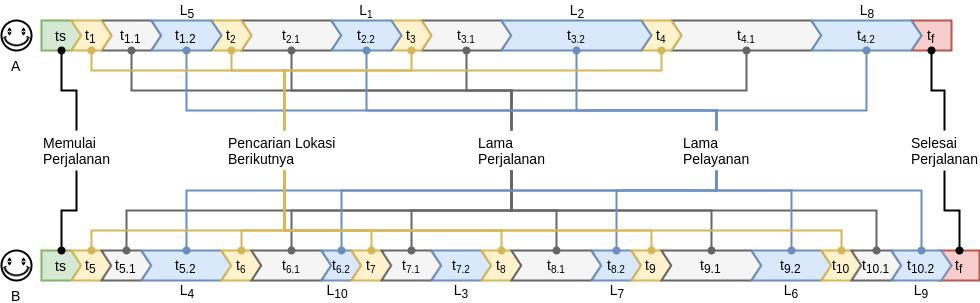
\includegraphics[width=\textwidth]{Resources/Images/illustration-timeline-realtime-mdvrp}
	\caption{Penerapan \textit{real time} MDVRP pada Permasalahan Alokasi Petugas Pencacahan}
	\label{fig:illustration-timeline-realtime-mdvrp}
\end{figure}

%-----------------------------------------------------------------------------%
\subsection{Garis Besar Sistem Usulan}
%-----------------------------------------------------------------------------%
Sistem usulan untuk rekomendasi lokasi pencacahan dirancang berdasarkan arsitektur \textit{publish/subscribe} yang terdiri dari 3 (tiga) komponen utama: \textit{publisher} rekomendasi, petugas pencacahan yang berperan sebagai \textit{subscriber}, dan \textit{message broker} yang berperan sebagai penerus pesan (\textit{message router}). \autoref{fig:system-overview} memberikan ilustrasi komponen yang menyusun sistem rekomendasi lokasi pencacahan usulan.


\begin{figure}[!]
	\centering
	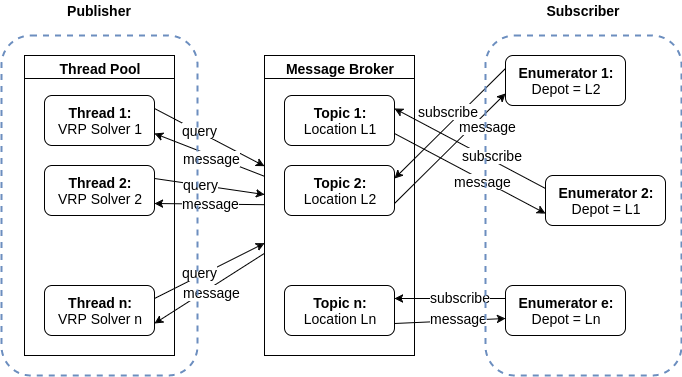
\includegraphics[width=\textwidth]{Resources/Images/system-overview}
	\caption{Garis Besar Sistem Usulan}
	\label{fig:system-overview}
\end{figure}


Komunikasi antara \textit{publisher} dan \textit{subscriber} terjadi atas dasar kesamaan topik/\textit{event}. Topik/\textit{event} didapatkan dari \textit{context} masing-masing pencacah. \textit{Context} dari pencacah dapat berupa jenis kelamin, tingkat pendidikan, umur, pengalaman, atau domisili/lokasi pencacah. Pada penelitian ini, \textit{current location} dari pencacah dipilih sebagai \textit{topik} karena bersifat \textit{unique}, dimana setiap lokasi pencacahan hanya akan dikunjungi oleh satu orang pencacah saja dan tidak akan ada lebih dari satu pencacah pada \textit{current location} yang sama.


%-----------------------------------------------------------------------------%
\subsection{\textit{Recommendation Publisher}}
\label{ssec:publisher}
%-----------------------------------------------------------------------------%
Berdasarkan konsep dasar mekanisme \textit{publish/subscribe}, \textit{publisher} akan mem-\textit{publish} informasi ke seluruh \textit{subscriber} tanpa melihat apakah \textit{subscriber} tersebut men-\textit{subscribe} topik dari informasi yang bersangkutan atau tidak. Akibatnya komunikasi yang berlangsung menjadi tidak efisien. Untuk mengatasi inefisiensi komunikasi ini, perlu dilakukan beberapa penyesuaian agar \textit{publisher} hanya akan mem-\textit{publish} informasi kepada \textit{subscriber} yang bersesuaian. 

Seorang \textit{subscriber} (petugas pencacahan) me-\textit{request} `lokasi pencacahan yang harus dituju' kepada \textit{publisher}. \textit{Request} ini tidak langsung diterima oleh \textit{publisher}, melainkan ditampung oleh \textit{message broker}. \textit{Publisher} akan mengecek \textit{message broker} secara berkala untuk mendeteksi ada atau tidaknya \textit{request} baru dengan menggunakan thread \textit{TopicWatcher} yang dideskripsikan pada \autoref{alg:topic-watcher} serta diilustrasikan dengan \textit{flowchart} pada \autoref{fig:topic-watcher}. 


\begin{algorithm}[!]
	\caption{TopicWatcher}
	\label{alg:topic-watcher}
	\begin{algorithmic}[1]
		\renewcommand{\algorithmicrequire}{\textbf{Input:}}
		\renewcommand{\algorithmicensure}{\textbf{Output:}}
		\REQUIRE $None$
		\ENSURE  $None$
		\\ $TP$ = Threadpool
		\\ $N$ = Number of locations
		\\ $M$ = Number of enumerators
		\WHILE {true}
			\STATE $C \leftarrow readAvailableTopicFromBroker()$	// channel
			\FOR {$m = 1$ to $len(C)$}
				\FOR {$n = 1$ to $N$}
					\IF {($C_m == L_n$)}
						\STATE $T_n = Thread(C_m, E_1...E_M, (unassigned) L_1...L_N)$	// E = enumerator
						\STATE submitThreadToThreadpool($T_n$, $TP$)
					\ENDIF
				\ENDFOR
			\ENDFOR
		\ENDWHILE
	\end{algorithmic}
\end{algorithm}



Untuk setiap \textit{request} yang diterima, \textit{publisher} akan menyiapkan sebuah \textit{thread} baru dengan menggunakan \textit{current location} dari \textit{subscriber}/petugas sebagai ID. \textit{Thread} ini dilengkapi dengan sebuah \textit{VRP solver procedure} (\autoref{alg:vrp-worker}) yang akan melakukan pencarian solusi/rute. Seluruh \textit{thread} dari masing-masing topik ditampung di dalam sebuah \textit{threadpool} yang menangani \textit{thread} berdasarkan urutan waktu kedatangan. Pada akhir proses pencacahan, dimana seluruh lokasi pencacahan sudah pernah di-\textit{request} dan di-\textit{assign} kepada petugas, ukuran \textit{threadpool} ini akan sama dengan jumlah seluruh topik yang tersedia. 


\begin{figure}[!]
	\centering
	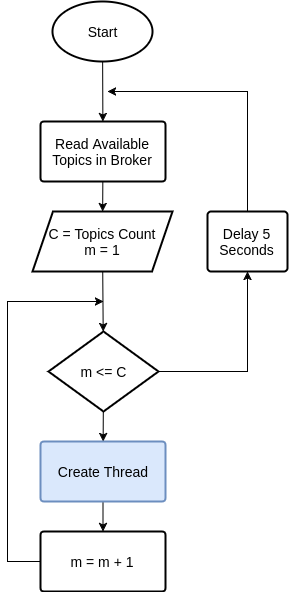
\includegraphics[width=6.3cm]{Resources/Images/topic-watcher}
	\caption{\textit{\textit{Flowchart} Topic Watcher}}
	\label{fig:topic-watcher}
\end{figure}


\textit{Thread-thead} di dalam \textit{threadpool} dieksekusi satu per satu sesuai dengan waktu kedatangan. Setiap eksekusi akan menjalankan \textit{VRPSolver procedure} yang melibatkan $M$ \textit{subscribers} (petugas pencacahan) dan \textit{unassigned} N lokasi pencacahan. \textit{VRPSolver procedure} harus mengikutsertakan seluruh \textit{subscriber} untuk memastikan diperolehnya solusi terbaik yang bersifat global (\textit{global best solution}). \autoref{fig:global-best-greedy-solution} memberikan ilustrasi algoritma \textit{Global Best Solution} dengan penjelasan sebagai berikut:
\begin{enumerate}
	\item Petugas A dan B masing-masing melakukan pencacahan pada lokasi 5 dan 6. \textit{Current location} mereka akan di-\textit{update} secara bersesuaian.
	\item Petugas B menyelesaikan pekerjaannya lebih cepat dari petugas A dan segera me-\textit{request} `lokasi pencacahan berikutnya'. Sistem kemudian menghitung `lokasi berikutnya' berdasarkan \textit{current location} dari petugas B. 
	\item Jika kalkulasi hanya melibatkan 1 petugas yang bersangkutan saja, maka \textit{VRPSolver procedure} akan merekomendasikan lokasi terdekat dari \textit{current location} petugas B, yakni lokasi 7. Namun, solusi yang dibuat berdasarkan sudut pandang lokal (\textit{local best solution}) seperti ini, dapat `merugikan' petugas lain yang tidak ikut dalam penghitungan. 
	\item Sebagai gambaran, misalkan saat A selesai melakukan pencacahan dan me-\textit{request} `lokasi berikutnya', lokasi 7 sudah tidak \textit{available} lagi bagi A. Rekomendasi terbaik yang bisa diberikan oleh sistem adalah lokasi 1 yang memiliki jarak yang cukup jauh dari A. 
	\item Rekomendasi yang lebih tepat bisa diperoleh jika \textit{VRPSolver procedure} mengikutsertakan seluruh petugas dalam penghitungan rute, analisis terhadap \textit{current location} dari seluruh petugas, menghasilkan \textit{global best solution} dimana petugas B akan mendapatkan lokasi 3 dan petugas A akan mendapatkan lokasi 7. 

\end{enumerate}

  Proses pencarian solusi akan berakhir ketika sudah tidak ada lagi lokasi pencacahan yang berstatus \textit{unassigned}. \textit{VRP Solver Procedure} dijelaskan secara lebih rinci pada \autoref{ssec:vrp-solver}.	\color{black}


\begin{figure}[!]
	\centering
	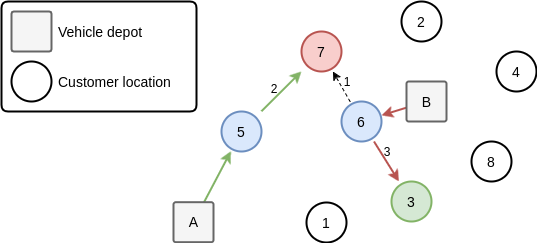
\includegraphics[width=12cm]{Resources/Images/global-best-greedy-solution}
	\caption{\textit{Algoritma \textit{Global Best Solution}}}
	\label{fig:global-best-greedy-solution}
\end{figure}


\begin{algorithm}[!]
	\caption{VRPSolver Procedure}
	\label{alg:vrp-worker}
	\begin{algorithmic}[1]
		\renewcommand{\algorithmicrequire}{\textbf{Input:}}
		\renewcommand{\algorithmicensure}{\textbf{Output:}}
		\REQUIRE $T$
		\ENSURE  $None$
		
		\WHILE {true}
			\STATE $T$ = popFirstThreadOrWaitNewThreadFromThreadpool()
			\STATE $R$ = VRPSolver($T$)
			\FOR {$j = 1$ to $len(R)$}
				\STATE $r$ = publish($C_{R_j}$, $R_j$)
				\IF {($r > 0$)}
					\STATE cancelSolver($T_j$)
				\ELSIF {($C_{T_i} \notin C_{R_j}$)}
					\STATE $T_i = Thread(C_{T_i}, V_m, (unassigned) E_1...E_N)$
				\ENDIF
			\ENDFOR
		\ENDWHILE		
	\end{algorithmic}
\end{algorithm}


Jumlah rute yang dihasilkan oleh \textit{VRPSolver} berkisar antara 1 (satu) hingga $M$ rute, dimana M merujuk pada jumlah petugas pencacahan yang mengirimkan \textit{request}. \color{red} --> subscript i merujuk pada apa? petugas pencacah kan? diganti m aja gmn? Terus didalam algoritma ada simbol T. apa itu? modifikasi simbol huruf menyesuaikan dg isi paragraf. \color{black} Setiap rute $R_m$ $(1 \leq m \leq M)$ yang dihasilkan oleh \textit{VRPSolver} akan di-\textit{publish} kepada petugas $m$ yang merupakan \textit{subscriber} topik (lokasi) $C_n$ $(1 \leq n \leq N)$. \color{red} --> prevsent: berarti 1 rute = 1 topik = 1 petugas, bener g??? jumlah rute = jumlah petugas \color{black}. Setelah solusi diteruskan kepada \textit{subscriber}, \textit{message broker} akan memberikan informasi tentang jumlah \textit{subscriber} yang menerima \color{red} --> menerima atau memesan???? \color{black} pesan kepada \textit{publisher}, tetapi identitas dari penerima tetap tidak diketahui. \color{red} --> lho kok message broker baru menghubungi publisher setelah solusi disampaikan ke subsrciber sih? kan harusnya message broker menghubungi publisher dulu, baru solusinya bisa diterusin ke subscriber??? \color{black}. Jika rute $R_i$ memiliki satu atau lebih penerima pesan, maka \textit{thread} yang memiliki ID $C_{n}$ \color{red} --> atau $C_{n_i}$ ??? \color{black} akan dianulir \color{red} --> knp kalo cm punya 1 subscriber juga ikut dibatalkan? jelasin lagi. aku lupa\color{black}. Pembatalan ini dilakukan agar solusi/rute yang telah diterima oleh \textit{subscriber} tidak dikalkulasi ulang. \color{red} --> prevsent: kalimat ini rasanya masih kurang. perlu sedikit lebih diperjelas lagi \color{black}


Pada praktiknya, dapat terjadi suatu kondisi dimana di antara rute-rute yang dihasilkan oleh \textit{VRPSolver}, tidak terdapat rute untuk topik/lokasi $C_{n}$ \color{red} --> atau $C_{n_i}$ ??? terus siapa yg sebenernya pnya ID? thread atau \textit{VRPSolver} ??? \color{black}. Pada kondisi demikian, topik $C_n$ \color{red} --> atau $C_{n_i}$ ??? \color{black} akan diantrikan kembali dengan masih melibatkan $(unassigned) N$ lokasi namun hanya 1 subscriber $m$ yang bersangkutan saja. Ini dilakukan untuk memberikan jaminan bahwa akan selalu ada solusi/rute untuk setiap topik $C_n$ \color{red} --> atau $C_{n_i}$ ??? \color{black}.


\begin{figure}[!]
	\centering
	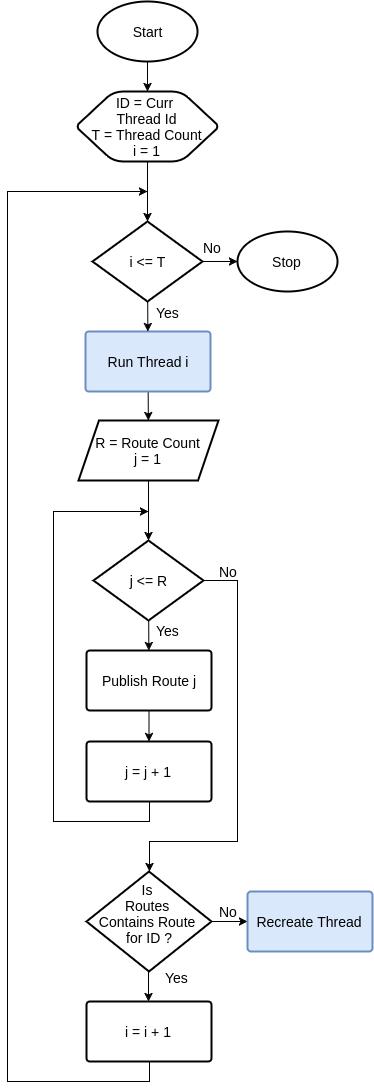
\includegraphics[width=\textwidth]{Resources/Images/recommendation-publisher}
	\caption{\textit{VRP Worker}}
	\label{fig:recommendation-publisher}
\end{figure}


Seperti yang telah dijelaskan pada \color{red} subsection xxx ??? \color{black}, karakteristik  \textit{loose coupling} memberikan fleksibilitas \color{red} fleksibilitas dalam artian??? \color{black} kepada mekanisme \textit{publish/subscribe}.  

Akan tetapi, keunggulan ini juga menjadi salah satu kelemahan dari mekanisme ini. Ketidaktahuan \textit{publisher} terhadap identitas \textit{subscriber} menyebabkan \textit{current location} dari setiap \textit{subscriber} tidak dapat diketahui. Untuk itu, diperlukan sebuah mekanisme yang dapat digunakan untuk pertukaran informasi antara \textit{publisher} dan \textit{subscriber}. Pada penelitian ini akan digunakan \textit{shared-memory} yang akan digunakan untuk menyimpan informasi \textit{current location} dari seluruh \textit{subscriber}, dan \textit{publisher} dapat mengaksesnya untuk mengetahui \textit{current location} dari setiap \textit{subscriber}.


Arsitektur \textit{publish/subscribe} merupakan sebuah arsitektur yang bersifat \textit{loose coopling}, dimana antara \textit{publisher} dan \textit{subscriber} tidak saling mengetahui \citep{muhl_large-scale_2002}. Salah satu konsekuensinya, ketika seorang pencacah melakukan \textit{subscribe}, pada saat solusi diperoleh pencacah tersebut sudah terputus dari \textit{broker}. Untuk itu diperlukan mekanisme \textit{caching}, sehingga pada saat pencacah terkoneksi kembali dengan \textit{broker}, maka solusi yang terdapat pada \textit{cache} dapat langsung di\textit{pusblish}.


%Proses di atas akan terus berulang sampai seluruh lokasi telah di\textit{assign} kepada \textit{subscriber}. \autoref{fig:publisher-algorithm} mengilustrasikan \textit{workflow} dari algoritma yang digunakan pada \textit{recommendation publisher}.
%
%
%\begin{figure}[!]
%	\centering
%	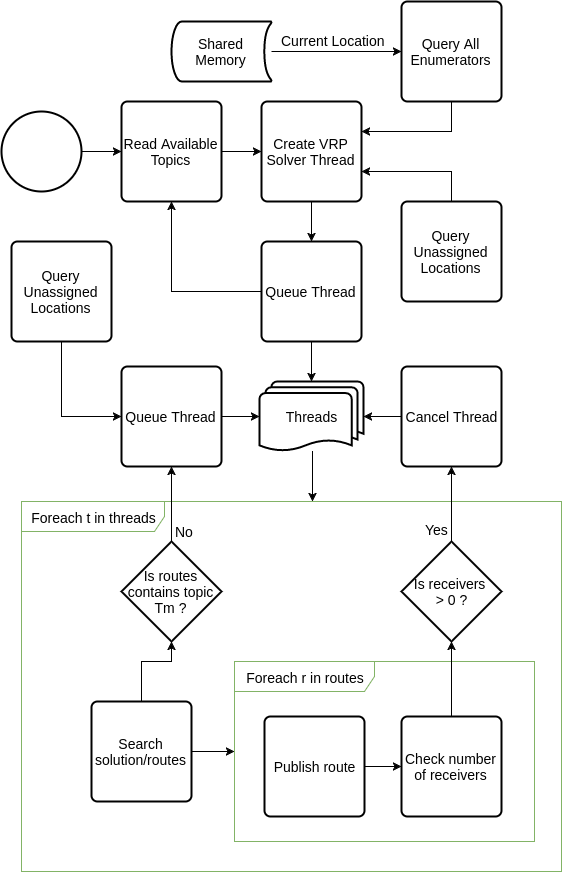
\includegraphics[width=12cm]{Resources/Images/publisher-algorithm}
%	\caption{Publisher Workflow}
%	\label{fig:publisher-algorithm}
%\end{figure}


%-----------------------------------------------------------------------------%
\subsection{\textit{VRP Solver}}
\label{ssec:vrp-solver}
%-----------------------------------------------------------------------------%
VRP solver merupakan sebuah modul yang digunakan dalam pencarian solusi/rute yang akan dikunjungi oleh setiap kendaraan. Vrp solver dipanggil dari setiap \textit{thread} dalam \textit{thread pool} (\autoref{alg:vrp-worker}). Terdapat beberapa algoritma yang dapat digunakan untuk menyelesaikan permasalahan MDVRP, seperti: tabu search \cite{cordeau_tabu_1997}, adaptive large neighborhood search  \citep{pisinger_general_2007}, fuzzy logic guided genetic algorithm \citep{lau_application_2010}, paralel iterated tabu search \citep{cordeau_parallel_2012}, hybrid algorithm combining iterated local search and set partitioning \citep{subramanian_hybrid_2013}, hybrid genetic algorithm with adaptive diversity control \citep{vidal_implicit_2014}, hybrid granular tabu search \citep{escobar_hybrid_2014}, dan cooperative coevolution algorithms (CoEAs) \citep{de_oliveira_cooperative_2016}. Pada penelitian ini akan digunakan \textit{coevolutionay algorithms} (CoEAs), karena algoritma CoEAs menghasilkan nilai \textit{mean solution values} yang kompetitif dengan waktu pemrosesan yang relatif rendah dibandingkan algoritma yang lain.


Langkah-langkah yang digunakan pada implementasi algoritma CoEAs pada VRP solver adalah sebagai berikut:
\begin{enumerate}
\item Definisi masalah \\
Masalah yang didefinisikan pada algoritma CoEAs sama seperti permasalahan MDVRP umumnya. Data yang diikutsertakan meliputi kendaraan sejumlah $M$ beserta masing-masing kapasitasnya $D_i$ dan konsumen sejumlah $N$ beserta masing-masing \textit{demand} $d_i$. Setiap lokasi $i, i \in (M \cup N)$ dilengkapi dengan koordinat $(x_i, y_i)$. Biaya untuk setiap kombinasi lokasi $c_{ij}$ juga diikutsertakan dalam permasalahan yang didefinisikan, dimana $i, j \in (M \cup N)$. Terdapat dua macam cara yang dapat digunakan dalam menghitung biaya, yaitu: \textit{euclidean}, dan \textit{Google location API}. Pada metode \textit{euclidean}, biaya dapat diasumsikan sebagai jarak antar lokasi, sementara pada metode \textit{Google location API} dapat digunakan waktu tempuh sebagai biaya.
\item Dekomposisi masalah \\
Pada CoEAs, terdapat beberapa spesies yang akan saling bekerja sama untuk membentuk solusi/rute terbaik. Pada implementasinya, masalah yang didefinisikan diatas kemudian didekomposisi menjada beberapa sub-masalah, dimana masing-masing sub-masalah akan merepresentasikan sebuah spesies.
\item Evolusi \\
Setelah terbentuk beberapa spesies, masing-masing individu dalam spesies tersebut akan berevolusi. Evolusi terjadi secara iteratif dalam beberapa generasi. Setiap kali generasi baru terbentuk, maka generasi tersebut akan dievaluasi dengan membandingkannya dengan generasi terbaik yang pernah ada sebelumnya. Jika generasi baru lebih baik, maka generasi tersebut diterima dan generasi terbaik akan diperbarui. Jumlah iterasi yang diperlukan dalam kasus ini akan dibatasi dengan batasan waktu. Iterasi akan berhenti setelah 60 detik, atau 40 detik tanpa perubahan generasi terbaik. Setelah iterasi terhenti, maka generasi terbaik akan menjadi solusi yang digunakan.
\end{enumerate}


%-----------------------------------------------------------------------------%
\subsection{\textit{Message Broker}}
\label{ssec:message-broker}
%-----------------------------------------------------------------------------%
\textit{Message broker} adalah sebuah komponen yang bertanggung jawab dalam menyalurkan (\textit{routing}) pesan dari \textit{publisher} ke \textit{subscriber} sesuai dengan topik yang di\textit{subscribe} \citep{banavar_efficient_1999}. Suatu sistem \textit{publish/subscribe} dapat memiliki \textit{single broker} maupun \textit{multi broker}. Pada arsitektur \textit{single broker}, seluruh \textit{subscriber} dan \textit{publisher} terkoneksi pada satu \textit{broker}, sementara pada \textit{multi broker}, setiap \textit{subscriber} maupun \textit{publisher} dapat terkoneksi pada broker terdekat. Arsitektur \textit{multi depot} ini juga disebut dengan \textit{distributed pub/sub system} \citep{muhl_large-scale_2002}, seperti ilustrasi pada Gambar \ref{fig:pub_sub_distributed_ilustration}. Adapun rancangan yang diusulkan akan menerapkan arsitektur terdistribusi, dikarenakan lokasi pencacahan secara geografis tersebar.


\begin{figure}[!]
	\centering
	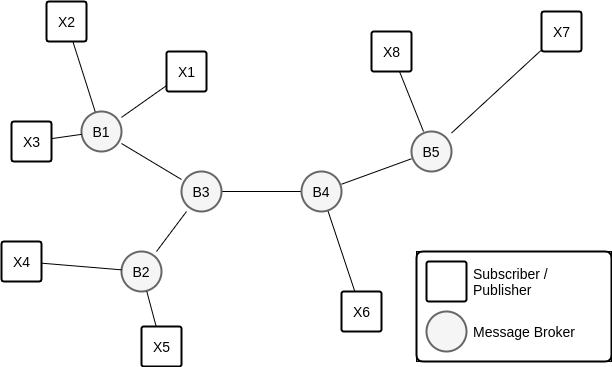
\includegraphics[width=9cm]{Resources/Images/pub_sub_distributed_ilustration}
	\caption{Arsitektur \textit{Publish-Subscribe} terdistribusi}
	\label{fig:pub_sub_distributed_ilustration}
\end{figure}


%#############################################################################%
\begin{comment}
%-----------------------------------------------------------------------------%
\subsection{\textit{Search Algorithm}}
%-----------------------------------------------------------------------------%
Terdapat berbagai variasi algoritma untuk menyelesaikan permasalah TSP maupun VRP, antara lain: genetic algorithm, simmulated annealing, tabu search, particle swarm optimization, harmony search, quantum annealing, greedy 2-opt, dll. Pada pengujian yang dilakukan dengan kasus single-salesman dengan menggunakan 3 (tiga) kriteria: \textit{mean quality}, \textit{dispersion of quality}, dan \textit{time needed to reach the optimum}, simmulated annealing menghasilkan solusi yang paling berkualitas, sementara tabu search merupakan yang paling baik dari sisi performance \citep{antosiewicz_choice_2013}.


%-----------------------------------------------------------------------------%
\subsection{\textit{Greedy Strategy}}
%-----------------------------------------------------------------------------%
Algoritma \textit{greedy} adalah suatu algoritma yang menentukan solusi optimal berdasarkan kondisi saat ini, atau disebut dengan \textit{local optimum}. Algoritma greedy dapat meminimalisir waktu komputasi dalam pencarian solusi global. Pada kasus \textit{travelling salesman problem}, strategi greedy dapat dikatakan dengan "pada setiap tahap, kunjungi kota yang paling dekat dengan lokasi salesman yang belum dikunjungi" \citep{paul_e._black_greedy_2005}. 


Pada metode MTSP, diperoleh lebih dari satu solusi, dimana masing-masing solusi diperbandingkan. Perbandingan dilakukan berdasarkan \textit{cost} keseluruhan, dimana solusi dengan \textit{cost} terkecil adalah solusi terbaik.


Penentuan solusi terbaik dengan membandingkan \textit{cost} keseluruhan tidaklah tepat. \textit{Cost} ditentukan dengan satuan waktu, sementara salah satu komponen utama yang dominan adalah \textit{service time}. Karena \textit{service time} tidak tersedia, maka membandingkan keseluruhan waktu akan menjadi bias. Hipotesis yang ditawarkan adalah membandingkan setiap solusi dengan total \textit{cost} untuk lokasi pertama dari masing-masing pencacah saja, karena lokasi pertama tidak terpengaruh dengan \textit{service time}, seperti algoritma dalam Kode \ref{lst:proposed_best_solution_algorithm}.


\begin{listing}
	\caption{Algoritma Solusi Terbaik}
	\label{lst:proposed_best_solution_algorithm}
	\begin{minted}[showspaces=false,breaklines=true]{python}
Let E be all enumerators
Let L be all locations
Run MTSP with enumerators E and locations L
Let S be all solutions from MTSP
Let Cs be an empty dict
For each solution s in S do
	Let R be all routes in solution s
	Let C be 0
	For each route r in R do
		Let J be all jobs in route r
		Let fj be first job in J
		Let cfj be cost of first job fj
		Add C with cjf
	Put C in dict Cs with key solution s
	
Let element in dict Cs with the least value be the best solution
	\end{minted}
\end{listing}


Algoritma \ref{lst:proposed_best_solution_algorithm} merupakan rekomendasi lokasi pertama untuk setiap pencacah. Selanjutnya pencacah dapat melakukan pengumpulan data pada lokasi tersebut sampai selesai, dengan \textit{service time} bervariasi, sehingga waktu selesai pencacahan berbeda-beda antar pencacah. Setiap pencacah yang telah menyelesaikan pengumpulan data, dapat melakukan \textit{subscribe} solusi yang baru kepada \textit{broker}, seperti algoritma pada Kode \ref{lst:proposed_subscribe_solution_algorithm}. Setiap kali broker mendapati adanya \textit{subscribers}, maka \textit{broker} akan mencari solusi baru dengan metode MTSP. Solusi yang dicari hanya menyertakan \textit{subscribers} saja, dan meng-\textit{exclude} lokasi yang telah dikunjungi, seperti algoritma pada Kode \ref{lst:proposed_subscribers_best_solution_algorithm}.


\begin{listing}
	\caption{Algoritma \textit{Subscribe Solution}}
	\label{lst:proposed_subscribe_solution_algorithm}
	\begin{minted}[showspaces=false,breaklines=true]{python}
Let SS be an empty list
For each e in enumerators E do
	If enumerator e has finished enumerating do
		Exclude location l enumerated by e from locations L
		Add e in list of subscribers SS
	\end{minted}
\end{listing}


\begin{listing}
	\caption{Algoritma Solusi Terbaik untuk \textit{Subscribers}}
	\label{lst:proposed_subscribers_best_solution_algorithm}
	\begin{minted}[showspaces=false,breaklines=true]{python}
While locations L is not empty do
	Run MTSP with enumerators SS and locations L
    Let S be all solutions from MTSP
    Let Cs be an empty dict
    For each solution s in S do
	    Let R be all routes in solution s
	    Let C be 0
	    For each route r in R do
		    Let J be all jobs in route r
		    Let fj be first job in J
		    Let cfj be cost of first job fj
		    Add C with cjf
	    Put C in dict Cs with key solution s
	
    Let Bs as element in dict Cs with the least value
    Publish Bs to all subscribers SS
    Set subscribers SS to empty list
	\end{minted}
\end{listing}


%-----------------------------------------------------------------------------%
\subsection{\textit{Publish/Subscribe Paradigm}}
%-----------------------------------------------------------------------------%








\section{Garis Besar Perancangan}

Alur kerja perancangan dimulai dengan dengan mengidentifikasi blok sensus yang akan dilakukan pendataan padanya, serta menentukan jumlah pencacah yang akan digunakan. Kedua permasalahan ini tidak akan dibahas terlalu mendalam dalam penelitian ini. Lokasi pencacahan telah ditentukan dalam fase perancangan sensus dan survei, mengikuti sebuah metodologi tertentu. Sementara jumlah pencacahan juga telah ditentukan, mengikuti jumlah sampel dan berbagai persyaratan tertentu, seperti waktu dan biaya.


Selanjutnya, setiap pencacah akan dialokasikan kepada blok sensus yang akan dicacah dengan menggunakan metode MTSP, sebagaimana diformulasikan oleh \citep{bektas_multiple_2006}, dengan ketentuan setiap pencacah dapat memulai dan mengakhiri pada \textit{depot} yang berbeda-beda. Setelah model diperoleh, setiap pencacah akan mengunjungi lokasi pertama dari rekomendasi. Setelah selesai kunjungan, lokasi akan disimpan dalam \textit{tabu list} dengan menggunakan metode pub-sub \citep{chen_efficient_2003}. Model baru akan digenerate setiap kali terdapat \textit{request} dari salah satu pencacah. Setiap kali model di-\textit{generate}, \textit{tabu search} \citep{glover_tabu_1989, glover_tabu_1990} yang memanfaatkan \textit{tabu list} akan digunakan untuk memastikan tidak terdapat \textit{conflict}. Setelah model baru selesai di-\textit{generate}, maka mudel akan di-\textit{publish} kepada setiap pencacah yang telah men-\textit{subscribe}.


\begin{figure}[!]
    \centering
    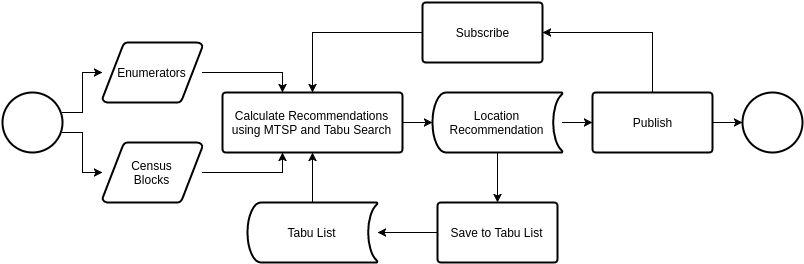
\includegraphics[width=\textwidth]{Resources/Images/design_overview}
    \caption{Garis Besar Sistem Usulan}
    \label{fig:design_overview}
\end{figure}


\section{Penyusunan Rekomendasi}

Pada tahap perumusan rekomendasi, input data yang terdiri dari data pencacah dan data blok sensus akan dioleh menjadi rekomendasi path yang harus dikunjungi. Proses penyusunan rekomendasi menggunakan metode \textit{Multiple Travelling Salesman Problem} (MTSP), yang merupakan pengembangan dari metode klasik \textit{Travelling Salesman Problem} (TSP).


Metode MTSP yang digunakan dalam masalah ini memiliki beberapa \textit{requirements}, antara lain:

\begin{itemize}
\item Jumlah \textit{depot} \\
MTSP dapat menggunakan lebih dari satu depot, dengan $ m_{j} $ \textit{salesman} untuk setiap depot $ j $. Pada permasalahan ini menggunakan \textit{non-fixed destination}, sehingga pencacahan tidak perlu kembali ke lokasi dimana pencacahan dimulai.
\item Jumlah \textit{salesman} \\
Jumlah \textit{salesman} yang digunakan dapat berupa \textit{fixed number} $ m $, atau dinamis dengan dibatasi jumlah maksimal $ max(m) $. Pada permasalahan ini digunakan \textit{fixed number} $ m $ pencacah.
\item \textit{Fixed charges} \\
Jika jumlah \textit{salesman} dinamis, maka bisa juga masing-masing \textit{salesman} dibatasi dengan sejumlah biaya tertentu. Pada permasalahan ini tidak digunakan \textit{fixed charges}.
\item Waktu kunjungan (\textit{time windows}) \\
\textit{Time windows} merepresentasikan waktu yang dihabiskan selama kunjugan dalam sebuah \textit{node}. Pada kasus ini \textit{time windows} tidak dapat ditentukan karena tidak tersedianya informasi, sehingga dianggap tidak menggunakan \textit{time windows}.
\end{itemize}


Requirements di atas, secara global dapat disederhanakan dalam tabel-tebel berikut. Tabel \ref{tbl:enumerators_overview} menunjukkan rancangan pencacah beserta koordinat \textit{depot}-nya, sementara Tabel \ref{tbl:census_blocks} menunjukkan rancangan blok sensus beserta koordinat dan \textit{time windows}-nya. Dalam fakta lapangan, jarak antara satu blok sensus dengan blok sensus yang lain tidaklah setara. Bisa jadi secara koordinat memiliki jarak yang berdekatan, tetapi secara akses tidaklah mudah. Untuk itu diperlukan sebuah tabel tambahan, yaitu tabel \textit{cost-matrix}, sebagaimana Tabel \ref{tbl:cost_matrix}. \textit{Cost} yang dimaksud disini adalah segala metrik yang dapat digunakan sebagai penimbang (\textit{weight}), misalnya: biaya, jarak, atau waktu tempuh.


\begin{table}[]
\centering
\caption{Table Pencacah}
\label{tbl:enumerators_overview}
\begin{tabular}{@{}lcc@{}}
\toprule
\multirow{2}{*}{Pencacah} & \multicolumn{2}{l}{\textit{Depot Coordinate}} \\ \cmidrule(l){2-3} 
                          & X                 & Y                \\ \midrule
Pencacah 1                & 20.0              & 20.0             \\
Pencacah 2                & 20.0              & 20.0             \\
Pencacah 3                & 30.0              & 40.0             \\
Pencacah 4                & 30.0              & 40.0             \\
...                       &                   &                  \\
Pencacah m                & x                 & y                \\ \bottomrule
\end{tabular}
\end{table}


\begin{table}[]
\centering
\caption{Tabel Blok Sensus}
\label{tbl:census_blocks}
\begin{tabular}{@{}lccc@{}}
\toprule
\multirow{2}{*}{Blok Sensus} & \multicolumn{2}{c}{Koordinat Lokasi} & \multirow{2}{*}{Time Windows} \\ \cmidrule(lr){2-3}
                             & X                 & Y                &                               \\ \midrule
001B                         & 62.0              & 63.0             & 0                             \\
002B                         & 63.0              & 69.0             & 0                             \\
003B                         & 46.0              & 10.0             & 0                             \\
004B                         & 61.0              & 33.0             & 0                             \\
...                          &                   &                  &                               \\
n                            & x                 & y                & 0                             \\ \bottomrule
\end{tabular}
\end{table}


\begin{table}[]
\centering
\caption{Table \textit{Cost-Matrix}}
\label{tbl:cost_matrix}
\begin{tabular}{@{}|c|c|c|c|c|c|c|@{}}
\toprule
        & 001B & 002B & 003B & 004B & ... & BS ke-n \\ \midrule
001B    & -    & 5    & 2    & 2    &     & ...     \\ \midrule
002B    &      & -    & 4    & 2    &     & ...     \\ \midrule
003B    &      &      & -    & 7    &     & ...     \\ \midrule
004B    &      &      &      & -    &     & ...     \\ \midrule
...     &      &      &      &      & -   & ...     \\ \midrule
BS ke-n &      &      &      &      &     & -       \\ \bottomrule
\end{tabular}
\end{table}


Tabel \textit{cost-matrix}, selain dapat didefinisikan secara manual (berdasarkan hasil survei atau perkiraan \textit{subject matter}), dapat juga didekati dengan menggunakan Google Directions API \citep{google_google_2016}. \textit{Request} yang digunakan menggunakan standar REST API, sementara \textit{response} yang ditampilkan dalam format JSON. Listing \ref{lst:google_direction_api_request} menunjukkan contoh \textit{request}, dan Gambar \ref{fig:google_direction_api_response} menunjukkan contoh \textit{response} dari Google Direction API.








%Gambar \ref{fig:mtsp_solution_example} berikut menunjukkan hasil rekomendasi dengan MTSP.
%
%
%\begin{figure}[!]
%    \centering
%    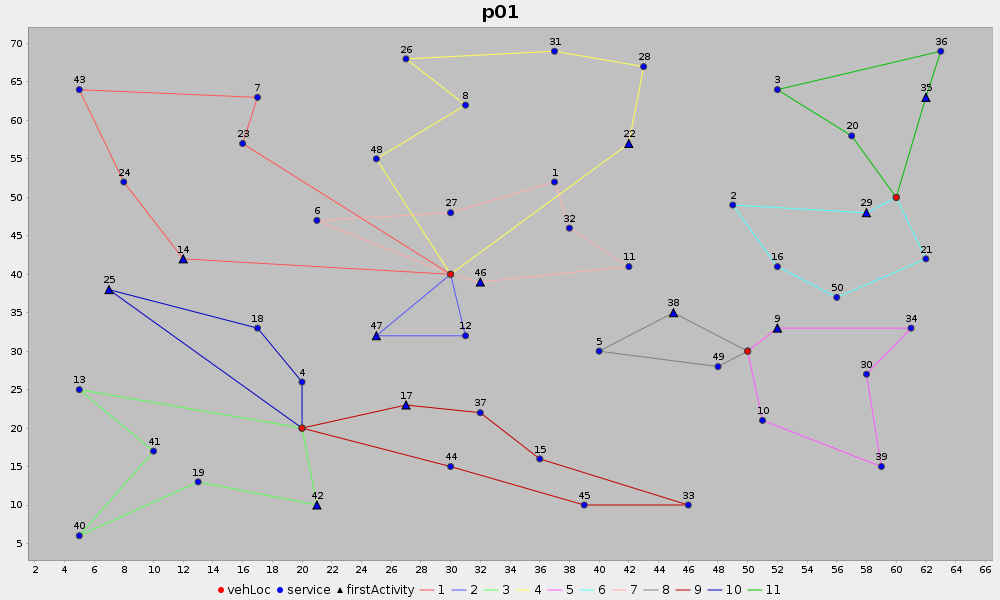
\includegraphics[width=\textwidth]{Resources/Images/mtsp_solution_example}
%    \caption{Contoh Hasil Rekomendasi}
%    \label{fig:mtsp_solution_example}
%\end{figure}


\section{Penyusunan \textit{Conflict Resolution}}


\section{\textit{Publish-Subscribe} Rekomendasi}
\end{comment}
%#############################################################################%
